\documentclass[10pt]{article}

\usepackage[T1]{fontenc}
\usepackage{geometry}
\usepackage{amsmath, amssymb, amsthm}
\usepackage{bm}
\usepackage{cancel}
\usepackage{xcolor}
\usepackage{graphicx}
\usepackage{caption}
\usepackage{subcaption}
\usepackage{hyperref}

\title{Mathematical Methods II - Assignment III}
\author{Satvik Saha}
\date{}

\geometry{a4paper, margin=1in}
\setlength\parindent{0pt}
\renewcommand{\labelenumi}{(\alph{enumi})}
\renewcommand\CancelColor{\color{red}}
% \renewcommand\qedsymbol{$\blacksquare$}
\newcommand\ve[1]{\boldsymbol{#1}}
\newcommand\ppx[1]{\frac{\partial #1}{\partial x}}
\newcommand\ppt[1]{\frac{\partial #1}{\partial t}}
\newcommand\pp[3][]{\frac{\partial^{#1}{#2}}{\partial {#3}^{#1}}}
\newcommand\ddx[1]{\frac{d #1}{d x}}
\newcommand\ddt[1]{\frac{d #1}{d t}}
\newcommand\dd[3][]{\frac{d^{#1}{#2}}{d {#3}^{#1}}}
\newcommand\norm[1]{\left\lVert#1\right\rVert}
\newcommand\grad[1]{\ve{\nabla}#1}
\newcommand\divg[1]{\ve{\nabla}\cdot#1}
\newcommand\curl[1]{\ve{\nabla}\times#1}
\newcommand\lapl[1]{\nabla^2 #1}

\begin{document}
        \par\textbf{IISER Kolkata} \hfill \textbf{Assignment III}
        \vspace{3pt}
        \hrule
        \vspace{3pt}
        \begin{center}
                \LARGE{\textbf{MA 2102 : Mathematical Methods II}}
        \end{center}
        \vspace{3pt}
        \hrule
        \vspace{3pt}
        Satvik Saha, \texttt{19MS154}\hfill\today
        \vspace{20pt}
        \subsection*{Partial Differential Equations (M.L. Boas, Chapter 13)}
        \paragraph{Section 1. Problem 2.}
        \begin{enumerate}
                \item Show that the expression $u = \sin(x - vt)$ describing a sinusoidal wave satisfies the wave equation
                \[
                        \lapl{u} = \frac{1}{v^2}\pp[2]{u}{t}.
                \]
                Show that in general, $f(x - vt)$ and $f(x + vt)$ satisfy the wave equation, where $f$ is any function with a second derivative. \\

                \textit{Solution.} Note that in one dimension, the laplacian $\lapl{}$ is simply the operator $\partial^2 /\partial x^2$
                (the other two spatial derivatives cause $u(x - vt)$ to vanish).
                Thus, we compute derivatives
                \[
                        \ppx{}u = \cos(x - vt),\quad\quad \pp[2]{}{x}u = \ppx{}\left(\ppx{}u\right) = -\sin(x - vt).
                \]
                \[
                        \ppt{}u = -v\cos(x - vt),\quad\quad \pp[2]{}{t}u = \ppt{}\left(\ppt{}u\right) = -v^2\sin(x - vt).
                \]
                Thus, $\ddot{u} = v^2 u''$ as desired, so $u$ does indeed satisfy the wave equation. \\

                For some general, twice differentiable function $f$, we can do the same. Let $f'$ and $f''$ denote the first and second
                derivatives of $f$ respectively. Then,
                \[
                        \ppx{}f(x \pm vt) = f'(x \pm vt),\quad\quad \pp[2]{}{x}f(x \pm vt) = \ppx{}\left(\ppx{}f(x \pm vt)\right) = f''(x \pm vt).
                \]
                \[
                        \ppt{}f(x \pm vt) = \pm vf'(x \pm vt),\quad\quad \pp[2]{}{t}f(x \pm vt) = \ppt{}\left(\ppt{}f(x \pm vt)\right) = v^2 f''(x \pm vt).
                \]
                Clearly, $\ddot{u} = v^2 u''$, where $u = f(x \pm vt)$ (these are actually two separate cases, which we present together for brevity).
                This means that $f(x \pm vt)$ are both solutions of the wave equation.

                \item Show that 
                \[
                        u(r, t) = \frac{1}{r} f(r \pm vt)
                \]
                both satisfy the wave equation in spherical coordinates. \\

                \textit{Solution.} We must verify that
                \[
                        \frac{1}{r^2}\pp{}{r}\left(r^2\pp{}{r}u\right) = \frac{1}{r}\pp[2]{}{r}(ru) = \frac{1}{v^2}\pp[2]{}{t}u.
                \]
                The first step follows by the product rule, which simplifies our work.
                \begin{align*}
                        \pp{}{r}\left(r^2\pp{}{r}u\right) - r\pp[2]{}{r}(ru)
                                &= 2r\pp{}{r}u + r^2\pp[2]{}{r}u - r\pp{}{r}\left(u + r\pp{}{r}u\right) \\
                                &= 2r\pp{}{r}u + r^2\pp[2]{}{r}u - 2r\pp{}{r}u - r^2\pp[2]{}{r}u \\
                                &= 0.
                \end{align*}
                Thus, we need only calculate
                \[
                        \frac{1}{r}\pp[2]{}{r}(r u) = \frac{1}{r}\pp[2]{}{r}f(r \pm vt) = \frac{1}{r}f''(r \pm vt), \quad\quad
                        \pp[2]{}{t}u = \frac{1}{r}\pp[2]{}{t}f(r \pm vt) = \frac{v^2}{r} f''(r \pm vt).
                \]
                Thus, $\ddot{u} = v^2u''$, so $f(r \pm vt) /r$ are indeed solutions of the wave equation.
        \end{enumerate}

        \paragraph{Section 4. Problem 2.} A string of length $\ell$ has a zero initial velocity and a displacement $y_0(x)$,
        described as
        \[
                y_0(x) = \begin{cases}
                        4hx /\ell, &\text{if } 0 \leq x \leq \ell/4, \\
                        2h - 4hx/\ell, &\text{if } \ell/4 < x \leq \ell/2, \\
                        0,      &\text{if } \ell/2 < x \leq \ell.
                \end{cases}
        \]
        Find the displacement as a function of $x$ and $t$. \\

        \textit{Solution.} We seek a solution $y(x, t)$ to the wave equation
        \[
                \pp[2]{}{x}y = \frac{1}{v^2}\pp[2]{}{t}y.
        \]
        We perform the separation of variable $y(x, t) = X(x)T(t)$, thus obtaining
        \[
                \frac{1}{X}\dd[2]{}{x}X = \frac{1}{v^2T}\dd[2]{}{t}T = \text{constant} = -k^2.
        \]
        Note that we chose $-k^2$ to ensure that our solutions do not diverge.
        Setting $kv = \omega$, we see that this is equivalent to the ODES
        \[
                X'' + k^2 X = 0, \qquad T'' + \omega^2 T = 0.
        \]
        Thus, our solutions look like $X(x) = A\cos{kx} + B\sin{kx}$, and $T(t) = C\cos{\omega t} + D\sin{\omega t}$.
        From the boundary conditions $y(0, t) = y(\ell, t) = 0$, we see that $A = 0$ and $k_n = n\pi/\ell$.
        From the initial condition $v(x) = y_0'(x) = 0$, we see that $T'(0) = \omega D = 0$. Thus, our solution is of the form
        \[
                y(x, t) \;=\; \sum_{n = 1}^\infty A_n\sin\frac{n\pi x}{\ell} \cos\frac{n\pi vt}{\ell}.
        \]
        The coefficients $A_n$ are obtained by observing that at $t=0$, we can write $y_0(x)$ as a sine series. Thus,
        \begin{align*}
                A_n &= \frac{2}{\ell}\int_0^\ell y_0(x) \sin\frac{n\pi x}{\ell}\: dx \\
                        &= \frac{2}{\ell}\int_0^{\ell/4} \frac{4hx}{\ell}\sin\frac{n\pi x}{\ell}\:dx +
                                \frac{2}{\ell}\int_{\ell/4}^{\ell/2} \left(2h - \frac{4hx}{\ell}\right)\sin\frac{n\pi x}{\ell}\:dx \\
                        &= \frac{2h}{n^2\pi^2}\left[4\sin\frac{n\pi}{4} - n\pi\cos\frac{n\pi}{4}
                                + 4\sin\frac{n\pi}{4} - 4\sin\frac{n\pi}{2} + n\pi\cos\frac{n\pi}{4}\right] \\
                        &= \frac{8h}{n^2\pi^2}\left[2\sin\frac{n\pi}{4} - \sin\frac{n\pi}{2} \right].
        \end{align*}
        Thus, we have our solution
        \[
                y(x, t) \;=\; \sum_{n = 1}^\infty \frac{8h}{n^2\pi^2}\left[2\sin\frac{n\pi}{4} - \sin\frac{n\pi}{2} \right] \sin\frac{n\pi x}{\ell} \cos\frac{n\pi vt}{\ell}.
        \]
        
        \paragraph{Problem 4.} Solve the previous problem if the initial displacement $y_0(x)$ is
        described as
        \[
                y_0(x) = \begin{cases}
                        4hx /\ell, &\text{if } 0 \leq x \leq \ell/4, \\
                        2h - 4hx/\ell, &\text{if } \ell/4 < x \leq 3\ell/4, \\
                        -4h + 4hx/\ell,      &\text{if } 3\ell/4 < x \leq \ell.
                \end{cases}
        \]
        Find the displacement as a function of $x$ and $t$. \\

        \textit{Solution.} We perform the separation of variables $y(x, t) = X(x)T(t)$ in the same manner as before, use the
        same boundary conditions to eliminate the cosine part of $X$, and use the initial conditions to eliminate the sine part of $T$.
        Thus,
        \[
                y(x, t) \;=\; \sum_{n = 1}^\infty A_n\sin\frac{n\pi x}{\ell} \cos\frac{n\pi vt}{\ell}.
        \]
        The only difference is in the coefficients $A_n$, which we recalculate as
        \[
                A_n = \frac{2}{\ell}\int_0^\ell y_0(x) \sin\frac{n\pi x}{\ell}\: dx.
        \]
        Note geometrically that $y_0(x) = -y_0(\ell - x)$, i.e.\ the reflection about $\ell/2$ is precisely the negative of the original curve. Thus,
        \[
                A_n = \int_{0}^{\ell/2} y_0(x)\sin\frac{n\pi x}{\ell} + y_0(\ell - x)\sin\frac{n\pi(\ell - x)}{\ell}\:dx
                        = \int_{0}^{\ell/2} y_0(x)(1 + \cos{n\pi})\sin\frac{n\pi x}{\ell}\:dx.
        \]
        We have used the identity
        \[
                \int_{0}^{2a} f(t)\:dt = \int_0^a f(t) + f(2a - t)\: dt.
        \]
        This means that $A_{2n+1} = 0$, otherwise, we use our previously calculated value of the integral to obtain
        \[
                A_{2n} = \frac{16h}{(2n)^2\pi^2}\left[2\sin\frac{2n\pi}{4} - \sin\frac{2n\pi}{2}\right] = \frac{8h}{n^2\pi^2}\sin\frac{n\pi}{2}.
        \]
        Thus, we have our solution
        \[
                y(x, t) \;=\; \sum_{n = 1}^\infty \frac{8h}{n^2\pi^2}\sin\frac{n\pi}{2}\sin\frac{2n\pi x}{\ell} \cos\frac{2n\pi vt}{\ell}.
        \]

        \paragraph{Problem 5.} A string of length $\ell$ is initially stretched straight; its ends are fixed for all $t$. At time $t = 0$,
        its points are given the velocity $V(x) = (\partial y/\partial t)_{t = 0}$ described by
        \[
                V(x) = \begin{cases}
                        2hx/\ell, &\text{if } 0 \leq x \leq \ell/2, \\
                        2h - 2hx/\ell, &\text{if } \ell/2 < x \leq \ell.
                \end{cases}
        \]
        Determine the shape of the string at time $t$.\\

        \textit{Solution.} We perform separation of variables $y(x, t) = X(x)T(t)$ again. The boundary conditions dictate that the cosine part
        of the spatial solution vanishes and $k_n = n\pi x/\ell$. However, since the string is perfectly flat initially,
        we make no judgement on the temporal part yet. Taking a time derivative, we see that the velocity function dictates $V(0) = V(\ell) = 0$.
        This means that the derivative of the temporal part, $-C\omega\sin{\omega t} + D\omega\cos{\omega t}$, must vanish at $0$ and $\ell$,
        so $D = 0$. Thus, our solution is of the form
        \[
                y(x, t) \;=\; \sum_{n = 1}^\infty A_n\sin\frac{n\pi x}{\ell} \sin\frac{n\pi vt}{\ell}.
        \]
        Taking a time derivative,
        \[
                \dot{y}(x, t) \;=\; \sum_{n = 1}^\infty A_n\frac{n\pi v}{\ell}\sin\frac{n\pi x}{\ell} \cos\frac{n\pi vt}{\ell}.
        \]
        Now we can set $t = 0$, whereby $\dot{y}(x, 0) = V(x)$ gives us the Fourier coefficients
        \[
                \frac{n\pi v}{\ell}A_n = \frac{2}{\ell}\int_0^\ell V(x) \sin\frac{n\pi x}{\ell}\: dx.
        \]
        If we note that $V(x) = V(\ell - x)$ due to symmetry, this simplifies the integral similarly to the previous problem, so
        \[
                \frac{n\pi v}{\ell}A_n = \frac{2}{\ell}(1 - \cos{n\pi})\int_0^{\ell/2} \frac{2hx}{\ell}\sin\frac{n\pi x}{\ell}\: dx = 
                        \frac{2h}{n^2\pi^2}(1 - \cos{n\pi})\left[2\sin\frac{n\pi}{2} - n\pi\cos\frac{n\pi}{2}\right].
        \]
        Note that $A_{2n} = 0$, and when $n$ is odd,
        \[
                A_n = \frac{2\ell}{n^3\pi^3v} (2)\left[2\sin\frac{n\pi}{2}\right] = \frac{8\ell}{n^3\pi^3 v}\sin\frac{n\pi}{2}.
        \]
        This vanishes anyways when $n$ is even. Thus, we have our solution
        \[
                y(x, t) \;=\; \sum_{n = 1}^\infty \frac{8h\ell}{n^3\pi^3v}\sin\frac{n\pi}{2}\sin\frac{n\pi x}{\ell} \sin\frac{n\pi vt}{\ell}.
        \]

        \paragraph{Problem 8.} Solve Problem 5 if the initial velocity is 
        \[
                V(x) = \begin{cases}
                        \sin{2\pi x/\ell}, &\text{if } 0 < x < \ell/2, \\
                        0, &\text{if } \ell/2 < x < \ell.
                \end{cases}
        \]\\

        \textit{Solution.} We use separation of variables $y(x, t) = X(x)T(t)$ and argue exactly the same as in Problem 5,
        obtaining the general solution
        \[
                y(x, t) \;=\; \sum_{n = 1}^\infty A_n\sin\frac{n\pi x}{\ell} \sin\frac{n\pi vt}{\ell}.
        \]
        To obtain the coefficients $A_n$, we take a time derivative and set $t=0$, so
        \[
                \frac{n\pi v}{\ell}A_n = \frac{2}{\ell}\int_0^\ell V(x) \sin\frac{n\pi x}{\ell}\: dx 
                        = \frac{2}{\ell} \int_0^{\ell/2} \sin\frac{2\pi x}{\ell}\sin\frac{n\pi x}{\ell}\:dx
                        = \frac{4}{(4 - n^2)\pi}\sin\frac{n\pi}{2}.
        \]
        Note that when $n = 2$, we must use L'H\^{o}pital's Rule, so
        \[
                A_2 = \frac{\ell}{2\pi v}\lim_{n \to 2} \frac{4}{(4 - n^2)\pi}\sin\frac{n\pi}{2} 
                        = \frac{\ell}{2\pi v}\lim_{n \to 2}\frac{-1}{n}\cos\frac{n\pi}{2}
                        = \frac{\ell}{4 \pi v}.
        \]
        Thus, we have our solution
        \[
                y(x, t) \;=\; \frac{\ell}{4 \pi v}\sin\frac{2\pi x}{\ell}\sin\frac{2\pi vt}{\ell} \,+\,
                \sum_{\substack{n = 1 \\n \neq 2}}^\infty \frac{4\ell}{n(4 - n^2)\pi^2 v}\sin\frac{n\pi}{2}\sin\frac{n\pi x}{\ell} \sin\frac{n\pi vt}{\ell}.
        \]

        \paragraph{Problem 12.} Let $f(x) = x - x^2$ on $(0, 1)$. Expand $f$ as a Fourier sine series and write the corresponding solutions
        for
        \begin{itemize}
                \item Temperature in a semi-infinite plate with the lower boundary fixed at $f$.
                \item Temperature in a rectangular plate of height $H$ with the lower boundary fixed at $f$.
                \item Heat flow in one dimension with initial temperature $f$.
                \item Particle in a box with initial condition $f$.
                \item A plucked string with initial shape $f$.
                \item A struck string with initial velocity $f$.
        \end{itemize}

        \textit{Solution.} We first write $f$ as a Fourier sine series
        \[
                f(x) = \sum_{n = 1}^\infty A_n\sin{n\pi x}.
        \]
        The coefficients are calculated as
        \[
                A_n = 2\int_0^1 f(x)\sin{n\pi x}\: dx = 2\int_0^1 (x - x^2)\sin{n\pi x}\:dx = \frac{4}{n^3\pi^3}(1 - \cos{n\pi}).
        \]
        We have used the integrals
        \begin{align*}
                \int_0^1 x\sin{n\pi x}\: dx &=  -\frac{x}{n\pi}\cos{n\pi x}\Big|_0^1 + \frac{1}{n\pi}\int_0^1 \cos{n\pi x}\: dx \\
                        &= -\frac{1}{n\pi}\cos{n\pi}. \\
                \int_0^1 x^2\sin{n\pi x}\:dx &= -\frac{x^2}{n\pi}\cos{n\pi x}\Big|_0^1 + \frac{1}{n\pi}\int_0^1 2x\cos{n\pi x}\:dx \\
                        &= -\frac{1}{n\pi}\cos{n\pi} + \frac{2x}{n^2\pi^2}\sin{n\pi x}\Big|_0^1 - \frac{2}{n^2\pi^2}\int_0^1 \sin{n\pi x}\: dx \\
                        &= -\frac{1}{n\pi}\cos{n\pi} - \frac{2}{n^3\pi^3}(1 - \cos{n\pi}).
        \end{align*}    
        Thus, $A_{n}$ vanishes for even $n$, and is equal to $8 /n^3\pi^3$ for odd $n$. With this, we directly use the equations
        indicated in the question to write our solutions (setting $\ell = 1$).
        \begin{enumerate}
                \item Temperature in a semi-infinite plate.
                \[
                        T \;=\; \sum_{n = 1}^\infty A_n e^{-n\pi y}\sin{n\pi x}. \tag{Eq 2.9}
                \]
                \item Temperature in a rectangular plate of height $H$.
                \[
                        T \;=\; \sum_{n = 1}^\infty A_n \left[\sinh{n\pi H}\right]^{-1}\sinh{n\pi (H - y)}\sin{n\pi x}. \tag{Eq 2.15}
                \]
                \item Heat flow in one dimension.
                \[
                        u \;=\; \sum_{n = 1}^\infty A_n e^{-(n\pi\alpha)^2 t}\sin{n\pi x}. \tag{Eq 3.12}
                \]
                \item Particle in a box.
                \[
                        \Psi \;=\; \sum_{n = 1}^\infty A_n e^{-iE_n t/\hbar}\sin{n\pi x},\qquad E_n = \frac{n^2\pi^2\hbar^2}{2m} \tag{Eq 3.26}
                \]
                \item Plucked string.
                \[
                        y \;=\; \sum_{n = 1}^\infty A_n \sin{n\pi x}\cos{n\pi vt}. \tag{Eq 4.7}
                \]
                \item Struck string.
                \[
                        y \;=\; \sum_{n = 1}^\infty \frac{A_n}{n\pi v} \sin{n\pi x}\sin{n\pi vt}. \tag{Eq 4.10}
                \]
        \end{enumerate}

        Computer plots of the above solutions are presented below. The code used to generate them can be found
        \href{https://gist.github.com/sahasatvik/b51aeafe25c88996d3d812580e04b09c}{here}.
        
        \begin{figure}[h]
        \centering
        \begin{subfigure}[b]{0.9\textwidth}
                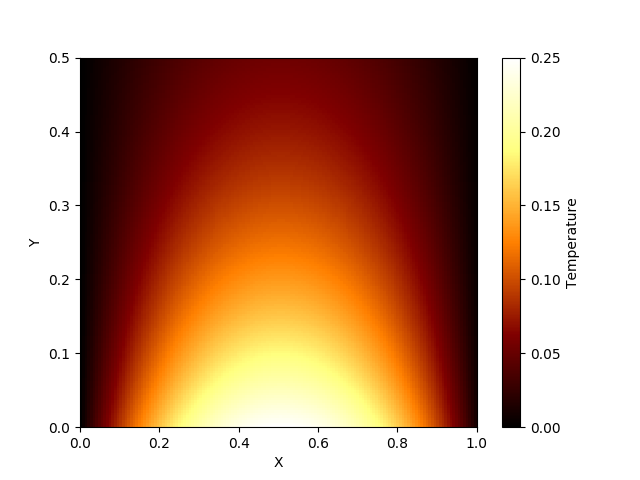
\includegraphics[width=\textwidth]{./semi_infinite_plate.png}
                \caption{Temperature in a semi-infinite plate}
        \end{subfigure}
        \end{figure}
        \begin{figure}[h]\ContinuedFloat
        \centering
        \begin{subfigure}[b]{0.9\textwidth}
                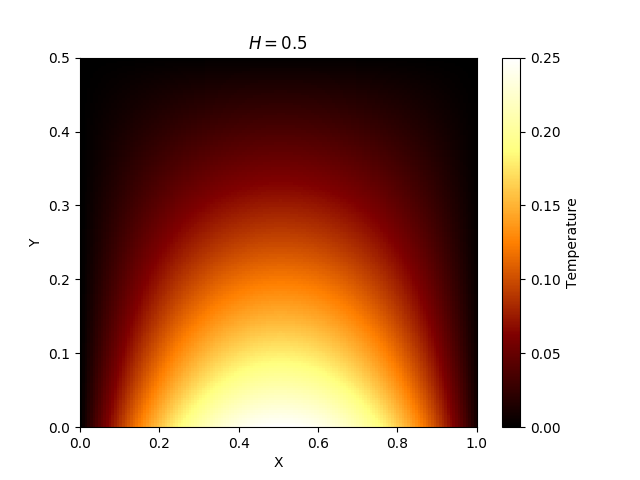
\includegraphics[width=\textwidth]{./finite_plate.png}
                \caption{Temperature in a rectangular plate, height $H$}
        \end{subfigure}
        \end{figure}
        \begin{figure}[h]\ContinuedFloat
        \centering
        \begin{subfigure}[b]{0.9\textwidth}
                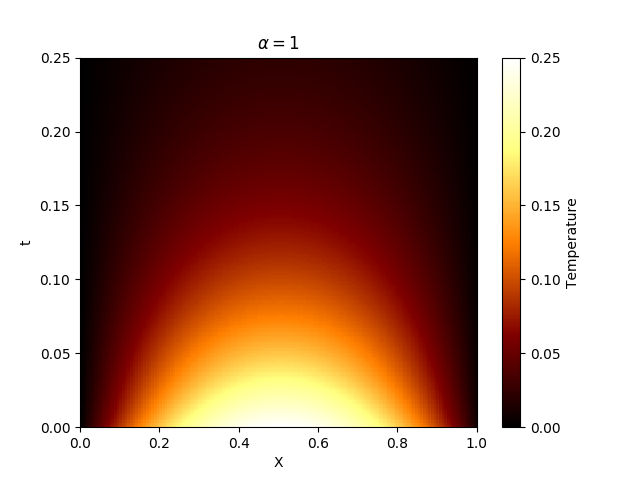
\includegraphics[width=\textwidth]{./heat_flow.png}
                \caption{Heat flow in 1D}
        \end{subfigure}
        \end{figure}
        \begin{figure}[h]\ContinuedFloat
        \centering
        \begin{subfigure}[b]{0.9\textwidth}
                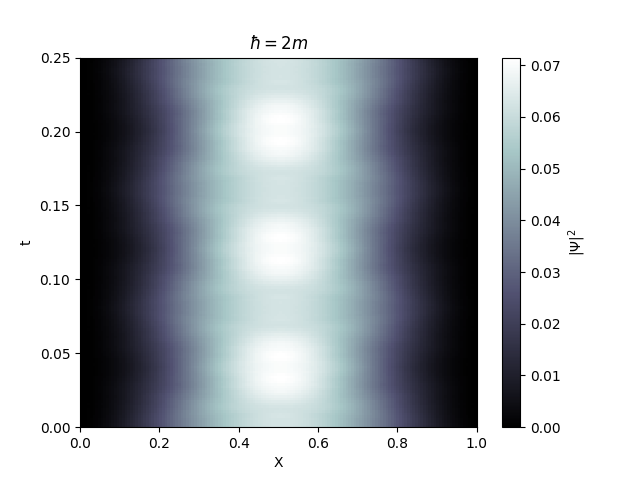
\includegraphics[width=\textwidth]{./particle_in_a_box.png}
                \caption{Particle in a box}
        \end{subfigure}
        \end{figure}
        \begin{figure}[h]\ContinuedFloat
        \centering
        \begin{subfigure}[b]{0.9\textwidth}
                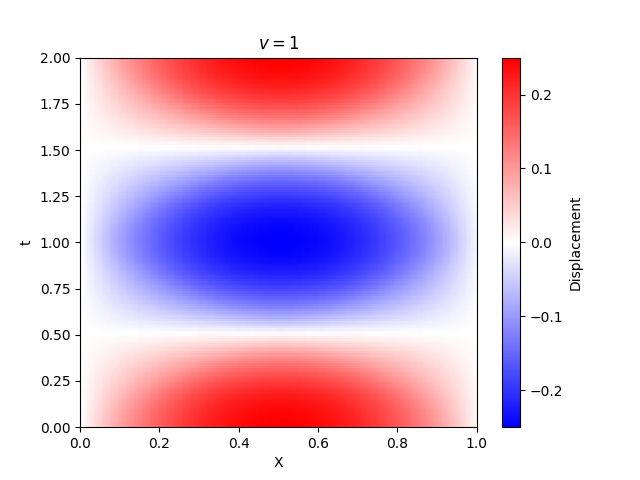
\includegraphics[width=\textwidth]{./plucked_string.png}
                \caption{Displacement of a plucked string}
        \end{subfigure}
        \end{figure}
        \begin{figure}[h]\ContinuedFloat
        \centering
        \begin{subfigure}[b]{0.9\textwidth}
                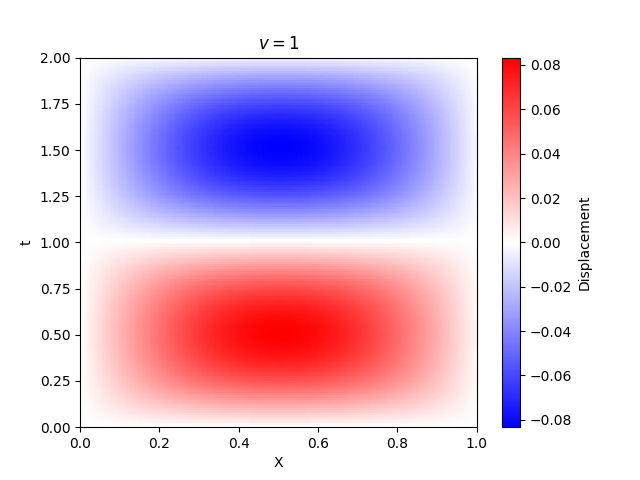
\includegraphics[width=\textwidth]{./struck_string.png}
                \caption{Displacement of a struck string}
        \end{subfigure}
        \caption*{Heatmaps of solutions.}
        \label{fig:plots}
        \end{figure}
\end{document}
